\section{Minimum spanning tree problem}

Given an undirected graph $G=(N,E)$ and a cost function, find a spanning tree $G_T=(N,T)$ of minimum total cost: 
\[\min_{T \in X} \sum_{e \in T}c_e\]
Here, $X$ is the set of all spanning trees of $G$. 
\begin{theorem}
    A complete graph with $n$ nodes $(n \geq 1)$ has $n^{(n-2)}$ spanning trees. 
\end{theorem}
To determine the spanning tree with the lowest total cost, we can employ an algorithm that incrementally constructs the spanning tree. 
The algorithm's fundamental concept is:
\begin{enumerate}
    \item Start by choosing any node arbitrarily and establish a connection to the nearest distinct node.
    \item Locate an unconnected node that is nearest to a connected node, and proceed to connect these two nodes. 
        Continue this process until all nodes are connected.
\end{enumerate}
\begin{example}
    Let's apply Prim's algorithm to the following graph:
    \begin{figure}[H]
        \centering
        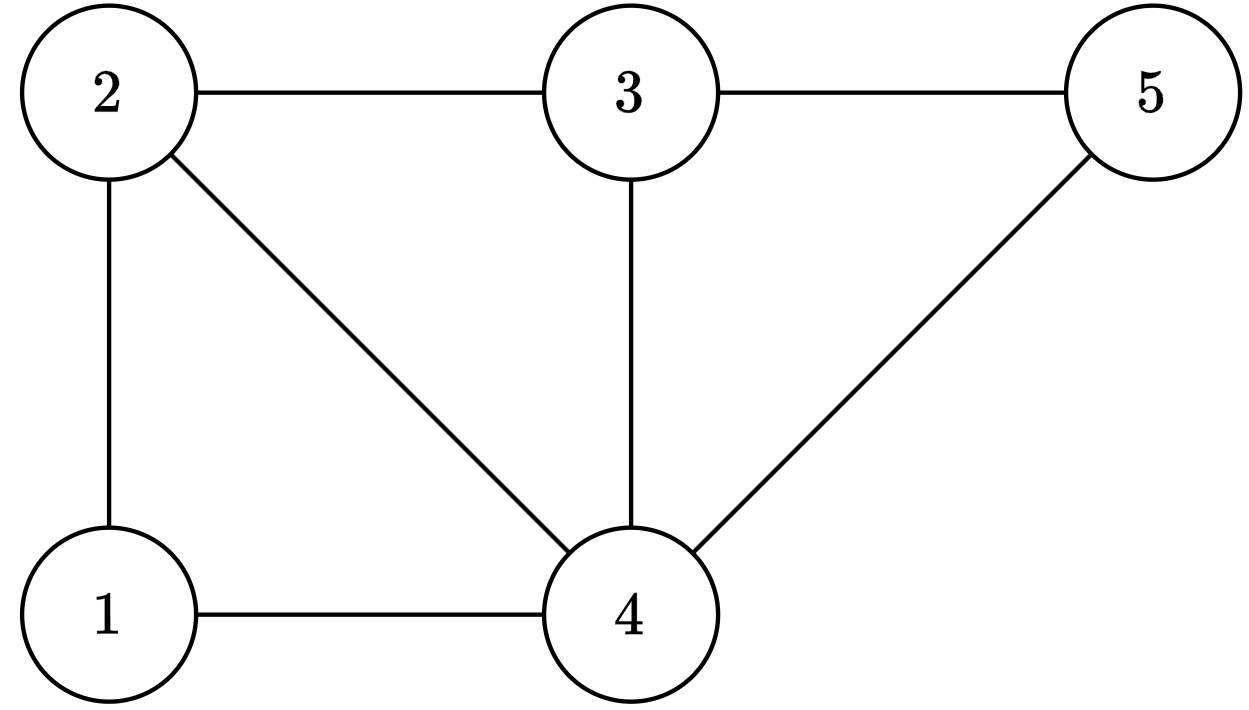
\includegraphics[width=0.3\linewidth]{images/sgraph.png}
    \end{figure}
    We start by selecting node 3 as our initial node. 
    Therefore, we have two sets: $S=\{3\}$ and $T=\{\varnothing\}$.
    Next, we follow these steps:
    \begin{itemize}
        \item The edge with the minimum cost connects nodes 3 and 4. 
            Now we have: 
            \begin{itemize}
                \item $S=\{3,4\}$.
                \item $T=\{\{3,4\}\}$.
            \end{itemize}
        \item The edge with the minimum cost connects nodes 1 and 4. 
            Now we have:
            \begin{itemize}
                \item $S=\{1,3,4\}$. 
                \item $T=\{\{3,4\},\{1,4\}\}$.
            \end{itemize}
        \item The edge with the minimum cost connects nodes 4 and 5. 
        Now we have: 
        \begin{itemize}
            \item $S=\{1,3,4,5\}$.
            \item $T=\{\{3,4\},\{1,4\},\{4,5\}\}$.
        \end{itemize}
        \item The edge with the minimum cost connects nodes 4 and 5. 
        Now we have:
        \begin{itemize}
            \item $S=N$.
            \item $T=\{\{3,4\},\{1,4\},\{4,5\},\{2,4\}\}$.
        \end{itemize}
    \end{itemize}
    In this case, the total cost is equal to $c(T)=6$. 
    Graphically, the resulting minimum spanning tree is as shown below:
    \begin{figure}[H]
        \centering
        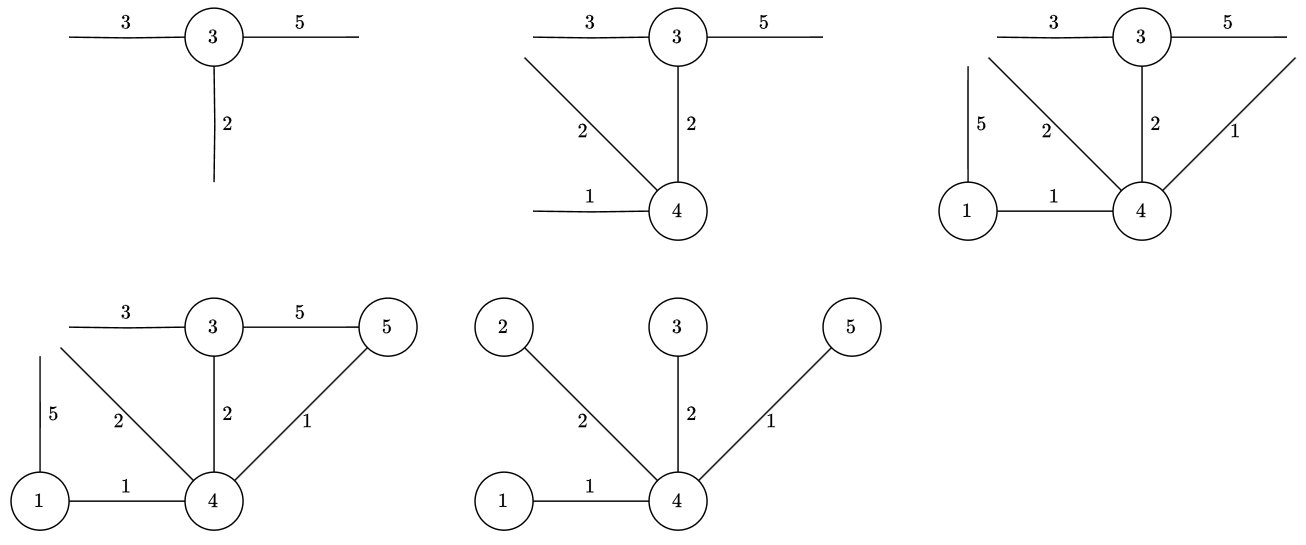
\includegraphics[width=0.8\linewidth]{images/MST.png}
    \end{figure}
\end{example}
\begin{algorithm}[H]
    \caption{Prim's algorithm for the minimum cost spanning tree problem}
        \begin{algorithmic}[1]
            \State $S \leftarrow \{u\}$
            \State $T \leftarrow \{\varnothing\}$
            \While {$\left\lvert T \right\rvert < n-1$}
                \State $\{u,v\}\leftarrow \textnormal{edge in } \delta(S) \textnormal{ of minimum cost}$
                \State $S \leftarrow S \cup \{v\}$
                \State $T \leftarrow T \cup \{u,v\}$
            \EndWhile
        \end{algorithmic}
\end{algorithm}
Where $u \in S$ and $v \in N-S$. 
The worst-case complexity is $O(n^2)$. 
\newpage
\begin{proposition}
    Prim's algorithm is exact. 
\end{proposition}        
The exactness does not depend on the choice of the first node nor on the selected edge of minimum cost in $\delta(S)$. 
\begin{property}
    Let $F$ be a partial tree contained in an optimal tree of $G$. 
    Consider $e\{u,v\}\in \delta(S)$ of minimum cost, then there exists a minimum cost spanning tree of $G$ containing $e$. 
\end{property}
\begin{proof}
    By contradiction, assume $T^{} \subseteq E$ is a minimum cost spanning tree with $F \subseteq T^{}$ and $e \notin T^{}$. 
    Adding edge $e$ to $T^{}$ creates the cycle $C$. 
    Let $f \in \delta(S) \cap C$.
    If $c_e=c_f$, then $T^{}\cup\{e\}-\{f\}$ is also optimal since it has same cost of $T^{}$.
    If $c_e<c_f$, then $c\left(T^{}\cup\{e\}-\{f\}\right)<C(T^{})$, hence $T^{*}$ is not optimal.
\end{proof}
\begin{proposition}
    Prim's algorithm is greedy. 
\end{proposition}     
At each step a minimum cost edge is selected among those in the cut $\delta (S)$ induced by the current set of nodes $S$. 
\begin{definition}[\textit{Cost decreasing edge}]
    Given a spanning tree $T$, an edge $e \notin T$ is cost decreasing if when $e$ is added to $T$ it creates a cycle $C$ with $C \subseteq T \cup \{e\}$ and $\exists f \in C-\{e\}$ such that $c_e<c_f$. 
\end{definition}
\begin{example}
    In the context of the given graph:
    \begin{figure}[H]
        \centering
        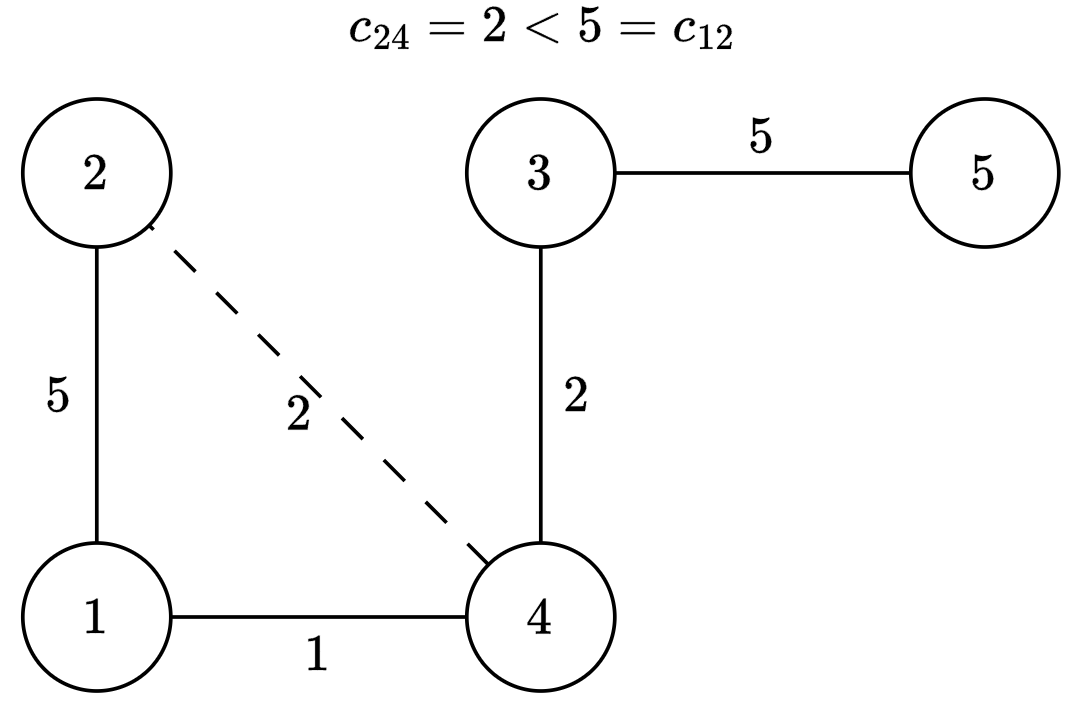
\includegraphics[width=0.4\linewidth]{images/costdecreasing.png}
    \end{figure}
    Since we have the equation:
    \[c(T \cup \{e\}-\{f\})=c(T)+c_e-c_f\]
    If edge $e$ is cost decreasing, it implies that:
    \[c(T \cup \{e\}-\{f\})<c(T)\]
\end{example}
\begin{theorem}
    A tree $T$ is of minimum total cost if and only if no cost decreasing edge exists. 
\end{theorem}

\begin{proof}
    We prove that if the tree is of minimum total cost if no cost decreasing edge exists.
    If a cost-decreasing edge exists, then $T$ is not of minimum total cost.
\end{proof}
\begin{proof}
    We prove that if no cost decreasing edge exists the tree is of minimum total cost.
    When there are no cost-decreasing edges, it implies that the spanning tree $T$ has the minimum total cost.
    Consider a minimum-cost spanning tree denoted as $T^{*}$, which is obtained through Prim's algorithm.
    It is possible to confirm that, by gradually exchanging one edge at a time, $T^{*}$ can be transformed step by step into $T$ without altering the overall cost.
    Consequently, we can conclude that $T$ is also an optimal solution.
\end{proof}
The optimality condition provides a means to confirm the optimality of a spanning tree $T$. 
To determine if $T$ is optimal, it is sufficient to examine whether each edge $e$ in the set $E-T$ is not a cost-decreasing edge.